% interactcadsample.tex
% v1.03 - April 2017

\documentclass[]{interact}

\usepackage{epstopdf}% To incorporate .eps illustrations using PDFLaTeX, etc.
\usepackage{subfigure}% Support for small, `sub' figures and tables
%\usepackage[nolists,tablesfirst]{endfloat}% To `separate' figures and tables from text if required

\usepackage{anyfontsize}% allow to choose any font size in section
\usepackage{natbib}% Citation support using natbib.sty
\usepackage{booktabs} % For prettier tables
\usepackage{graphicx} % For prettier tables
\usepackage{caption,booktabs} % For prettier tables (center the label)

\usepackage{graphicx} % insert figure
\graphicspath{ {./figures/} }

\captionsetup{justification = centering}
\usepackage{hyperref} % linke table to text

\usepackage{har2nat} % Allows to use harvard package with natbib https://mirror.reismil.ch/CTAN/macros/latex/contrib/har2nat/har2nat.pdf

% For citing with natbib, you may want to use this reference sheet: 
% http://merkel.texture.rocks/Latex/natbib.php

\usepackage{setspace}

\usepackage{pdfpages} % we can include pdf figures into the article

\usepackage{algorithm} % for algorithm box
\usepackage{algorithmicx} % for algorithm box
\usepackage{algpseudocode} % for algorithm box

\usepackage{colortbl} % for color table

\usepackage{algorithmicx} % for font size of algorithms
\usepackage{algpseudocode} % for font size of algorithms

\theoremstyle{plain}% Theorem-like structures provided by amsthm.sty

\newtheorem{theorem}{Theorem}[section]
\newtheorem{lemma}[theorem]{Lemma}
\newtheorem{corollary}[theorem]{Corollary}
\newtheorem{proposition}[theorem]{Proposition}

\theoremstyle{definition}
\newtheorem{definition}[theorem]{Definition}
\newtheorem{example}[theorem]{Example}

\theoremstyle{remark}
\newtheorem{remark}{Remark}
\newtheorem{notation}{Notation}

\begin{document}
	
    %\begin{titlepage}
	%	\begin{center}
	%		\vspace*{1.1cm}
	%		
	%		\Huge
	%		\textbf{Changepoint Detection in Social Networks: an Extension of the Relational Event Model}
			
	%		\vspace{1.8cm}
	%		\LARGE
	%		RESEARCH REPORT
			
	%		\vspace{1.8cm}
			
	%		\textbf{Hsuan Lee (9252568)}
			
	%		\vspace{1cm}
	%		Supervisors: 
			
	%		\vspace{0.5cm}
			
	%		Dr. Mahdi Shafiee Kamalabad 
			
	%		\& 
			
	%		Dr. Javier Garcia Bernardo
			
	%		\vspace{2cm}
	%		\Large
			
	%		\ Programme: MSBBSS
			
	%		\vspace{0.3cm}
			
	%		\emph{Department of Methodology \& Statistics}\\
			
	%		\vspace{0.3cm}
	%		Utrecht University\\
	%		the Netherlands\\
			
	%		\vspace{1.5cm}    
	%		\Large
	%		Date: 08.05.2023
			
	%		Candidate Journal: Social Networks
			
	%		FETC Case Number: 22-1870; 22-1871
		
	%	\end{center}
	%\end{titlepage}



    \begin{titlepage}
	
	    \raggedright % Add this line to left-align the content
	
	    \vspace*{-0.9cm}
	
	    \begin{figure}[H]
		    
\includegraphics[width=4.2cm]{UU_logo}
	    \end{figure}
	
	    \vspace*{1.4cm}
	
	    \rule{\linewidth}{0.1pt} % Add a solid bottom line
	
	    \vspace{0.3cm}
	    \large
	    \textbf{Research Master, Methodology \& Statistics} \\
	    \vspace{0.2cm}
	    \textbf{Utrecht University, the Netherlands}
	
	    \vspace{3cm}
    	\textbf{MSc Thesis, Hsuan Lee (9252568)} \\
	    \vspace{0.2cm}
	    \textbf{TITLE: Changepoint Detection in Social Networks: an Extension of the Relational Event Model} \\
	    \vspace{0.2cm}
	    \textbf{May 2023} \\
	
	    \vspace{3cm}
	    \textbf{Supervisors:} \\
	    \vspace{0.2cm}
	    \textbf{Dr.\emph{Mahdi Shafiee Kamalabad}} \\
	    \vspace{0.2cm}
	    \textbf{Dr.\emph{Javier Garcia Bernardo}} \\
	
	    \vspace{1.75cm}
	    \textbf{Second grader:} \\
	    \vspace{0.2cm}
	    \textbf{Dr.\emph{Gerko Vink}} \\
	
	    \vspace{1.75cm}
	    \textbf{Preferred journal of publication: Social Networks} \\
	    \vspace{0.2cm}
	    \textbf{Word count: 7618}
	
	    %\vspace{-0.2cm}
	    \rule{\linewidth}{0.1pt} % Add a solid bottom line
	
    \end{titlepage}



	
	\articletype{THESIS PROPOSAL}
	
	\vspace*{1cm}
	\hspace{-0.45cm}{\Large \textbf{Abstract}} \\
	
	\small{Time-stamped relationships dominate our lives. From scheduled meetings to social media interactions, the ebb and flow of our daily routines are dictated by time and the people around us. The Relational Event Model (REM) is a well-established model used to analyze time-stamped social interaction in a social network. The conventional REM assumes that the strength of endogenous and exogenous effects in the model is constant over the entire event history. This assumption can be unrealistic in real-world situations where social interaction can vary significantly between periods of time. For example, critical situations can fundamentally alter the communication between people, which is of key interest to social network researchers. However, the conventional REM cannot identify the number and locations of the time periods where the effects' strength changes abruptly. To fill this gap, we introduced three state-of-the-art changepoint detection algorithms (Bayesian Online Changepoint Detection (BOCPD), Pruned Exact Linear Time (PELT), and Binary Segmentation (BS)) into the REM structure to test and compare their effectiveness and performance. We first employed the moving window approach to segment the event history, which we called windows, and fit the REM on each window. By doing this, we could observe the dynamics of effects over time. We then utilized changepoint detection algorithms to detect changepoints across windows. Our analysis of synthetic data showed that BOCPD performed well in terms of precision, most of the windows it identified as containing changepoints were highly convincing. PELT was capable of revealing most of the windows containing changepoints in the network, but this came at a trade-off with its high number of false positives. BS was the least effective algorithm, it could not reveal as many windows containing changepoints as PELT, and it also lacked the high precision of BOCPD. We validated our findings using the Apollo 13 voice loop data, which provided similar results. Both BOCPD and PELT captured all the potential windows we hypothesized that included changepoints, while BS missed a few.} \\
	
	\hspace{-0.45cm}{\textbf{Keywords: }} \\
	\small{Social network, Relational Event Model, Moving Window approach, Changepoints detection, Binary Segmentation, Pruned Exact Linear Time, Bayesian Online Changepoint Detection Method} \\
	
	\newpage


	\section{\fontsize{14}{15}\selectfont Introduction} \label{sec:intro}
	
	\hspace{0.2cm} The Relational Event Model (REM) is a widely-used model for studying time-stamped social interactions and predicting future events in social networks. It uses factors such as gender, age, and inertia, known as ``effects," to parameterize the interaction rates between actors \cite{buttsRelationalEventFramework2008}. The REM assumes that the strength of these effects is constant over time, but in reality, social networks are dynamic and the strength of these effects can change over time. Identifying changepoints in the REM can help us understand when social network dynamics change qualitatively. For example, in a classroom setting, the social network may change over time based on students' interests, hobbies, or existing relationships. Identifying these changepoints can help teachers and administrators better support student engagement and social connections, ultimately leading to a more positive learning environment. \\
	
	As social networks are dynamic and can undergo changes in the strengths of the effects over time, it is important to identify changepoints in the REM to better understand the evolution of the network and underlying social dynamics. Changepoints represent sudden shifts in time series data that reflect transitions occurring between conditions \cite{sharmaTrendAnalysisChange2016}\cite{aminikhanghahiSurveyMethodsTime2017}, detecting them is essential in many domains, as evidenced by numerous studies. For example, Rauhameri and Salminen compared the performance of changepoint detection algorithms on IMS data from a portable ion mobility spectrometer \cite{rauhameriComparisonOnlineMethods2022}. Jarušková utilized a maximum type statistics to detect changepoints in hydrological and meteorological series \cite{jaruskovaProblemsApplicationChangePoint1997}. van den Burg and Williams evaluated and compared the performance of changepoint detection algorithms in general situations using 37 real-world time series data from diverse application domains \cite{burgEvaluationChangePoint2022}. In the social network area, Shafiee Kamalabad et al, suggested using Bayes Factor to infer changepoints in the REM \cite{shafieekamalabadWhatPointChange2023}. This approach uses the support of two hypotheses from the data to prove the existence of changepoints. However, there have been few studies on changepoint detection under the social network domain, especially in the REM framework. \\
	
	The aim of this study is to introduce changepoint detection algorithms into the REM structure. This is done to address the existing gap in REM's capability to detect changes in network dynamics. To accomplish this, we employ the moving window relational event model developed by Mulder and Leenders \cite{mulderModelingEvolutionInteraction2019}, which we refer to as MW-REM. The MW-REM mechanism involves delineating a specific duration of time (i.e., a window) that partially overlaps with the subsequent window. This window then slides over the entire event history, allowing us to observe fluctuations in the effects over time. To detect changepoints in the social network, We utilizes the effect fluctuations along the windows as input for the changepoint detection algorithms: Binary Segmentation (BS), Pruned Exact Linear Time (PELT), and Bayesian Online Changepoint Detection (BOCPD). These algorithms were identified as top performers in a comparison conducted by van den Burg and Williams \cite{burgEvaluationChangePoint2022} in a general application. It is important to note that due to the overlapping property of MW-REM, a changepoint may be involved in multiple consecutive windows. We refer to these windows as ``changepoint windows". \\
	
	In this study, we specifically investigate two main aspects: (1) the effectiveness and performance comparison of the three changepoint detection algorithms under the REM structure, and (2) proposing suitable application conditions for each algorithm based on our findings. To evaluate their feasibility and performance in the context of social network scenarios within MW-REM, we employ synthetic data to calculate metrics such as Confusion Matrix, Mean Squared Error (MSE), and Mean Signed Difference (MSD). We also test these algorithms on real-life social network data to assess their external validity. The combination of changepoint detection algorithms and MW-REM is applicable to any social network scenario, including communication in surgical rooms, interactions between teachers and students, as well as cooperation and competition between companies. The detection of changepoints can facilitate a better understanding of social dynamics, identify potential challenges as they arise, and inform future strategies based on data. \\ %The blueprint of our study is depicted in \autoref{Figure 1}. \\
    
    The thesis is structured as follows: In Methodology (\autoref{sec:method}), we introduce REM and MW-REM, followed by the three changepoint detection algorithms used in our study. Next, we explain how we utilize these algorithms on MW-REM, demonstrate how we simulate synthetic data, and model real-life data, i.e., the Apollo 13 voice loop data. Finally, we explain how we calculate metrics for the synthetic data to compare the algorithms. In Results and Discussion (\autoref{sec:results}), we present the effectiveness of the three changepoint detection algorithms on both synthetic and real-life data and compare their results. To aid understanding, we provide a list of abbreviations and mathematical symbols used in this study in \autoref{abbrev}.
    
    %\begin{figure}[H]
    %	\captionsetup{justification=raggedright}
    %	\captionsetup{labelfont={bf}, labelsep=space, font={footnotesize}}
    %	\renewcommand{\figurename}{Figure}
    %	\centering
    %	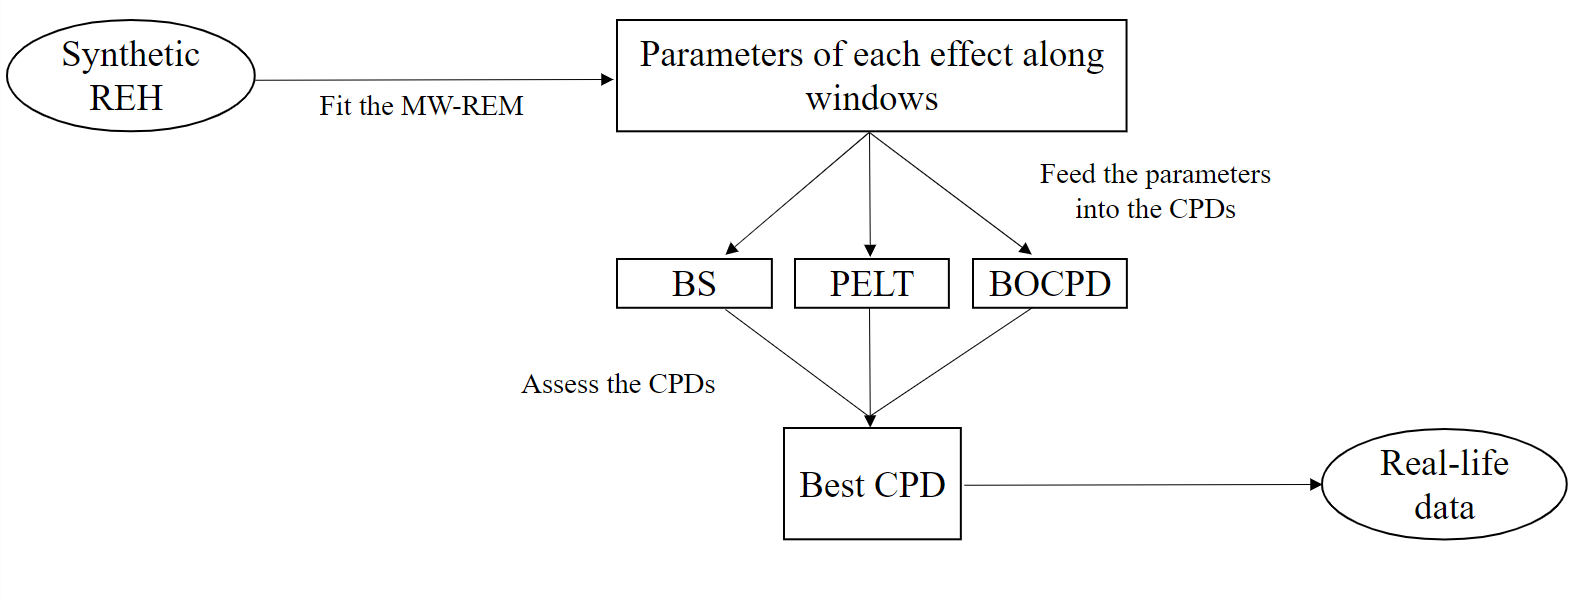
\includegraphics[width=11cm]{Flow_whole}
    %	\caption{\fontsize{8}{10}\selectfont Flowchart Depicting the Research Design of the Present Study}
    %	\label{Figure 1}
    %\end{figure}

    \begin{table}[H]
    	\captionsetup{justification=raggedright, singlelinecheck=true, labelfont={bf}, labelsep=space, font={footnotesize}, width=0.85\linewidth}
    	\centering
    	\renewcommand{\arraystretch}{1.1} % increase cell height by 50%
    	\scriptsize
    	\caption{Abbreviations and mathematical symbols.}
    	\begin{tabular}{ll}
    		\hline
    		\textit{\textbf{\begin{tabular}[c]{@{}l@{}}Abbreviations/\\ mathematical symbols\end{tabular}}} & \textit{\textbf{Decription}}                                  \\ \hline
    		\textit{REM}                                                                                    & Relational Event Model                                        \\
    		\textit{MW-REM}                                                                                 & Moving Window approach / Moving Window Relational Event Model \\
    		\textit{Changepoint window}                                                                     & a window that contains changepoint                            \\
    		\textit{REH}                                                                                    & Relational Event History data                                 \\
    		\textit{BS}                                                                                     & Binary Segmentation Changepoint Detection Algorithm           \\
    		\textit{PELT}                                                                                   & Pruned Exact Linear Time Changepoint Detection Algorithm      \\
    		\textit{BOCPD}                                                                                  & Bayesian Online Changepoint Detection Algorithm               \\
    		\textit{$(s,r)$}                                                                                & sender, receiver pair                                         \\
    		\textit{$R$}                                                                                    & risk set                                                      \\
    		\textit{$\beta_p$}                                                                              & parameter of effect $p$ / effects strength                    \\
    		\textit{$t$}                                                                                    & time $t$                                                      \\
    		\textit{$\lambda$}                                                                              & rate parameters                                               \\
    		\textit{$x_p$}                                                                                  & statistics of effect $p$                                      \\
    		%\textit{$C$}                                                                                    & cost function of  BS, and PELT                                \\
    		%\textit{$m$}                                                                                    & the number of changepoints                                    \\
    		%\textit{$\tau_i$}                                                                               & the location of a possible changepoint                        \\
    		\textit{OutdegreeSender}                                                                        & Outdegree of the Sender effect                                \\
    		\textit{IndegreeReceiver}                                                                       & Indegree of the receiver effect                               \\
    		\textit{TotaldegreeSender}                                                                      & Total degree of the sender effect                             \\
    		\textit{psABBA}                                                                                 & AB-BA pshift effect                                           \\
    		\textit{psABBY}                                                                                 & AB-BY pshift effect                                           \\
    		\textit{psABXA}                                                                                 & AB-XA pshift effect                                           \\
    		\textit{TP}                                                                                     & true positive                                                 \\
    		\textit{FP}                                                                                     & false positive                                                \\
    		\textit{FN}                                                                                     & false negative                                                \\
    		\textit{MSE}                                                                                    & Mean Squared Error                                            \\
    		\textit{MSD}                                                                                    & Mean Signed Difference                                        \\
    		\textit{$g$}                                                                                    & changepoint condition                                         \\ \hline
    	\end{tabular}
      \label{abbrev}
    \end{table}
	
	\section{\fontsize{14}{15}\selectfont Methodology} \label{sec:method}
	
	\subsection{Relational Event Model (REM)} \label{sec:REM}
	
	\hspace{0.28cm} The REM is an effective tool for modeling Relational Event History Data (REH), which at minimum involves sender, receiver, and time information, as shown in \autoref{Table 1}. By analyzing the impact of various effects on the social network, the REM enables us to understand the social interaction dynamic and forecast the timing and participants of the future events in the network \cite{buttsRelationalEventFramework2008}. This approach parameterizes both exogenous effects and endogenous effects. Exogenous effects are actor characteristics that do not depend on past interactions in the network, such as age or gender. Endogenous effects, on the other hand, depend on past interactions in the network, such as transitivity or inertia \cite{meijerink-bosmanDiscoveringTrendsSocial2022}. \\
	
	\begin{table}[H]
		\captionsetup{justification=raggedright, singlelinecheck=true, labelfont={bf}, labelsep=space, font={footnotesize}, width=0.85\linewidth}
		\centering
		\renewcommand{\arraystretch}{1.1} % increase cell height by 50%
		\small
		\caption{An example of Relational Event History Data, consisting of three flight crew members and their communication messages with timestamps.}
		\begin{tabular}{llll}
			\hline
			Time (hh,  mm, ss) & sender & receiver & message                                  \\ \hline
			13:14:05           & Patel  & Chen     & The weather conditions look good.        \\
			13:14:09           & Chen   & Patel    & Yes, it should be a smooth flight.       \\
			13:14:12           & Nguyen & Chen     & I've done my safety checks.              \\
			13:14:14           & Chen   & Nguyen   & Great job!                               \\ \hline
		\end{tabular}
		\label{Table 1}
	\end{table}
	
	To predict the next event in the network, the REM considers every possible sender-receiver combination $(s,r)$ as a potential occurrence at time $t$, and the collection of these pairs at time $t$ is named the risk set, denoted as $R(t)$. The risk set's size for each event is usually $N \times (N-1)$, where $N$ refers to the number of actors in the social network, as each actor can only be either a sender or a receiver, but not both. The REM models the event rate ($\lambda$) for each sender-receiver pair $(s,r)$ to predict which pair will be involved in the next event and when it will occur. The event rate is assumed to remain constant between the time of the present event and the time of the following event, the pair with a higher event rate in the risk set $R$ at time $t$ is more likely to occur in the next event. The probability of the $(s,r)$ taking place in the next event follows a multinomial distribution \cite{buttsRelationalEventFramework2008}, given by
	\begin{equation} \label{1}
		P \left((s,r) | t \right) = \dfrac{\lambda(s,r,t)} {\sum_{R(t)} \lambda(s,r,t)},
	\end{equation}
	where $\lambda(s,r,t)$ represents the event rate of a pair $(s,r)$ and $R(t)$ denotes the risk set for time $t$. \\
	
	The duration between two events follows an exponential distribution \cite{buttsRelationalEventFramework2008}, which is given by
	\begin{equation} \label{2}
		\Delta t \sim Exponential \left(\sum_{R(t)} \lambda(s,r,t) \right),
	\end{equation}
	where $\Delta t$ denotes the duration between two events. The higher the total event rate of the risk set, the shorter the $\Delta t$. \\
	
	The event rate is typically considered as a log-linear function of the statistics in REM with specific effects \cite{buttsRelationalEventFramework2008}, given by
	\begin{equation} \label{3}
		\log \lambda(s,r,t) = \sum_{p} \beta_p x_p(s,r,t),
	\end{equation}
	where $\beta_p$ represents the parameter of effects, which expresses the strength of one effect on the entire social network, and $x_p(s,r,t)$ denotes the statistics, which can be either an exogenous or endogenous effects. \\
	
	Despite the REM's outstanding capability in capturing social network dynamics and forecasting, its weakness lies in the assumption that the strength of all effects (i.e., $\beta_p$) remains constant throughout the entire event history. This assumption is unrealistic considering the dynamic property of social interactions. For instance, in a surgical room, unexpected situations such as a patient suddenly experiencing excessive bleeding can alter the communication dynamics among team members. The frequency and urgency of communication may increase as the team works to manage the situation and ensure the patient's safety. Therefore, assuming that effect strengths remain constant throughout the event history can result in inaccurate predictions and an incomplete understanding of social network dynamics. \\
	
	To overcome this shortcoming, in the next subsection, we will explain how the Moving Window approach works. Introduced by Mulder and Leenders in 2019 \cite{mulderModelingEvolutionInteraction2019}, this approach is particularly useful for analyzing social network dynamics and can assist researchers in tracking evolution in effect over time. In this thesis, we will utilize the moving window approach as input for our changepoint detection algorithms.
	
	\subsection{Moving Window-Relational Event Model (MW-REM)} \label{sec:MW-REM}
	
	\hspace{0.23cm} The Moving Window approach (MW) \cite{mulderModelingEvolutionInteraction2019} addresses the limitations of the REM by allowing for varying effect strengths over time. The MW involves setting up a fixed-size window, i.e., a fixed length of time, that slides over the entire Relational Event History (REH) data. Each window overlaps with the previous window, and the REM is fitted to each window (see \autoref{Figure 2}). We refer to this approach as MW-REM in this study. The MW-REM allows us to reveal the dynamics of each effect on the social network over time through the effect parameters ($\beta_p$) given in each window. It enables us to investigate the dynamic changes of the effect strengths in social networks, a feature not available in the original REM. However, one disadvantage of the approach is that it may not be able to identify drastic changes. To detect these changes, we integrate changepoint detection algorithms into the MW-REM framework. In the following subsection, we will discuss the changepoint detection algorithms we utilize and demonstrate how we apply them to the MW-REM.
	
    \begin{figure}[H]
    	\captionsetup{justification=raggedright}
    	\captionsetup{labelfont={bf}, labelsep=space, font={footnotesize}}
    	\renewcommand{\figurename}{Figure}
    	\centering
    	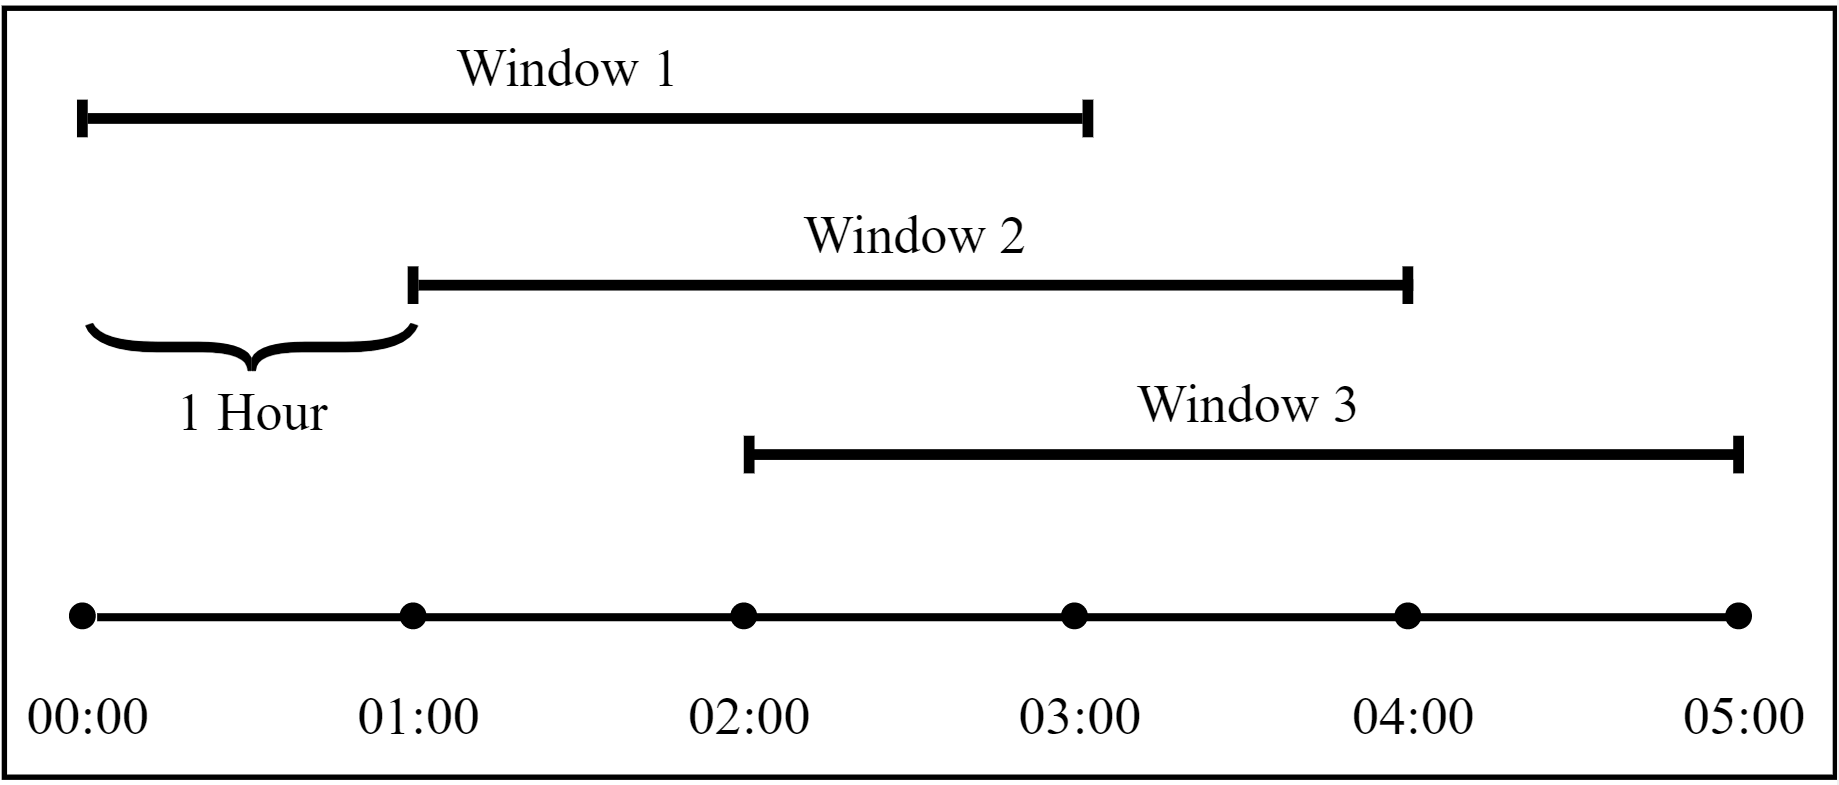
\includegraphics[width=13cm]{MW}
    	\caption{\fontsize{8}{10}\selectfont Example of Moving Window Approach: a window length of 1 hour with an overlap of $\frac{1}{3}$.}
    	\label{Figure 2}
    \end{figure}
    
	% add curly bracket for the plot
	\begin{picture}(0,0)
		\put(36,70.5){\makebox(137.5,4){\upbracefill}}
		\put(128.2,104.3){\makebox(137,4){\upbracefill}}
		\put(220.3,138){\makebox(137,4){\upbracefill}}
	%\put(100.8,99){\makebox(137,4){\upbracefill}}
	\end{picture}
	
	\subsection{Changepoint detection} \label{sec:CP detection}
	
	\hspace{0.2cm} Building upon the MW-REM discussed in the previous subsection, we aim to detect changepoints in the REH. As MW-REM divides the event history into partially overlapping sub-portions to fit the REM, it provides us with effect parameters ($\beta_p$) for each window over time, indicating the strength of each effect during that period, as shown in \autoref{3}. By fitting MW-REM to the event history, we obtain as many REMs as the fitting windows, and therefore the same number of effect parameters ($\beta_p$) as the number of fitting windows. \\
	
	We utilizes three changepoint detection algorithms for detecting changepoints in social networks: Binary Segmentation (BS), Pruned Exact Linear Time (PELT), and Bayesian Online Changepoint Detection (BOCPD). According to van den Burg and Williams \cite{burgEvaluationChangePoint2022}, these three changepoint detection algorithms were identified as top performers in a comparison in a general application. The comparison was based on criteria such as $F1$ scores and Segmentation covering metric. We chose these changepoint detection algorithms for their respective advantages and suitability for detecting changepoints in social networks, which can have abrupt changes over time. It is worth noting that changepoint detection algorithms can be classified into two categories, online and offline methods. Online methods aim to detect changes immediately in a real-time context, while offline methods examine changes retrospectively upon collection of complete data \cite{kendrickChangePointDetection2018}. In our study, BS is an offline method, PELT and BOCPD are online methods. The fundamental mechanisms of the three changepoint detection algorithm are presented in the following sections.
	
	\subsubsection{Binary Segmentation (BS)} \label{sec:BS}
	
	%\hspace{-0.55cm} \textbf{Binary Segmentation (BS)}\\
	
	\hspace{0.28cm} Binary Segmentation is a commonly used algorithm for detecting changepoints in heterogeneous time series data. The algorithm is based on a divide-and-conquer approach, which involves recursively splitting the time series into smaller segments until a segment is found that appears to be homogeneous with respect to a statistical property of interest, such as the mean or variance. Once a segment is found to be homogeneous, a changepoint is detected at the boundary between that segment and the previous one \cite{killickOptimalDetectionChangepoints2012}. \\
	
	The key idea behind Binary Segmentation is to minimize a cost function that penalizes the number of changepoints and the size of the segments. The cost function can be thought of as a trade-off between model complexity and goodness of fit. A more complex model with more changepoints may fit the data better, but it will also be more likely to overfit and capture noise in the data. On the other hand, a simpler model with fewer changepoints may underfit and miss important changes in the data. The most common cost function for multiple changepoint detection is given by
	\begin{equation} \label{4}
		\sum_{i = 1} ^{m + 1} \left[C(y_{({\tau_{i-1} + 1}):\tau_{i}}) \right] + \beta f(m),
	\end{equation}
	where $i$ denotes the order of a time point in a segment, $m$ indicates the number of changepoints, $\tau_i$ implies the location of a possible changepoint (i.e., time point $i$). And the m changepoints will divide the data into $m+1$ segments, with the $i$th segment contains $y_{({\tau_{i-1} + 1}):\tau_{i}}$. $C$ represents the cost function of a segment, $\beta f(m)$ serves as a penalty to prevent overfitting \cite{killickOptimalDetectionChangepoints2012}. \\
	
	To trade-off between accuracy and simplicity, BS starts with a single segment that spans the entire time series and recursively splits the segment into two smaller segments at the point that minimizes the cost function. This process continues until no further splits are possible, given by
	\begin{equation} \label{5}
		C(y_{1:\tau}) + C(y_{({\tau + 1}):n}) + \beta < C(y_{1:n}),
	\end{equation}
	In other words, BS searches for possible changepoints until there is no $\tau$ that meets the criteria. At this point, BS stops. Finally, the set of changepoints detected in each segment are merged to obtain the final set of changepoints.
	
	\subsubsection{Pruned Exact Linear Time (PELT)} \label{sec:PELT}
	
	%\hspace{-0.55cm} \textbf{Pruned Exact Linear Time (PELT)}\\
	
	\hspace{0.23cm} PELT is another algorithm for detecting changepoints in time series data. Like Binary Segmentation, PELT is a divide-and-conquer approach that recursively splits the time series into smaller segments. However, PELT is more efficient because its computational complexity is linear with respect to the length of the time series \cite{killickOptimalDetectionChangepoints2012}. \\
	
	The cost function used in PELT is similar to the one used in Binary Segmentation, and is given by \autoref{4}. However, the difference is that in PELT, the cost of each segment is computed recursively using the cost of the previous segment, which allows PELT to avoid recomputing the cost of the entire time series at each step of the algorithm. \\
	
	The key idea behind PELT is to iteratively remove candidate changepoints that do not significantly reduce the cost function in \autoref{4}. Specifically, PELT starts with a single segment that spans the entire time series, and then recursively splits the segment into smaller segments at the point that minimizes the cost function \cite{chapmanMetaAnalysisMetricsChange}. At each step, PELT evaluates the cost of adding a new changepoint between each pair of adjacent segments. If the cost of adding a new changepoint is not significant, the algorithm prunes the candidate changepoint and continues with the next pair of adjacent segments. This process is repeated until no further candidate changepoints remain. \\
	
	The final set of changepoints detected by PELT is obtained by merging the remaining candidate changepoints with the ones detected in each smaller segment. The resulting set of changepoints provides an exact solution that minimizes the cost function in \autoref{4} with the fewest possible number of changepoints.
	
	\subsubsection{Bayesian Online Changepoint Detection (BOCPD)} \label{sec:BOCPD}
	
	%\hspace{-0.55cm} \textbf{Bayesian Online Changepoint Detection (BOCPD)}\\
	
	\hspace{0.27cm} Unlike the BS and PELT, which rely on cost functions to identify changepoints, Bayesian Online Changepoint Detection (BOCPD) infers changepoints based on a Bayesian approach, which defines changepoints in terms of posterior probabilities, also known as run length probabilities, at time points. \\
	
	In BOCPD, the run length is a critical concept that represents the duration since the last detected changepoint. This concept is similar to the segments in PELT and BS. Whenever BOCPD detects a changepoint, the run length drops to 0, and the length is recalculated. To determine the changepoints, BOCPD computes the run length probabilities, which are posterior probabilities based on its posterior distribution for each time point. The run length probability consists of growth probabilities and changepoint probabilities. Growth probabilities indicate the probability that the data is generated from the same underlying distribution as the previous time points, while changepoint probabilities indicate the probability that a changepoint occurred at a particular time point. These probabilities are calculated using a Bayesian approach, which incorporates prior knowledge about the data generation process into the analysis. \\
	
	According to Adams and Mackay \cite{adamsBayesianOnlineChangepoint2007}, in order to reduce computational costs, it is suggested to set a cut-off point for estimating the run length probability. Typically, this cut-off point is defined as the total mass of the run length probability being less than $10^{-4}$. If the run length probability reaches such a cut-off point, the time point is determined as a changepoint. \\
	
	Overall, BOCPD starts by building the predictive distribution from the potential locations of changepoints, which reveals any prior knowledge regarding the data generation process. Based on the given predictive distribution, BOCPD computes the run length probability at a time point. As new data come in, the predictive distribution is continuously updated, and BOCPD iteratively runs the same procedure until no new data appear.
	
	\subsubsection{Changepoint detection procedures} \label{sec:our method}
	
	\hspace{0.27cm} In this section, we will discuss the settings used for each of the three changepoint detection algorithms we employed in our thesis, as well as the steps we took for changepoint detection based on the MW-REM structure. \\
	
	When using BS and PELT, selecting an appropriate statistical criterion to detect changepoints is crucial. For example, one statistical criterion for detecting changepoints is to look for significant changes in the mean or variance of the time series. However, the mean criterion is not robust to outlying observations, as noted by Dehling et al. \cite{dehlingRobustMethodShift2020}. The mean difference only detects changes in the mean value, assuming a constant variance. Similarly, variance difference only detects changes in the variance, assuming a constant mean. To improve changepoint identification, we consider changes in both the mean and variance when using BS and PELT. \\
	
	On the other hand, BOCPD does not rely on a specific statistical criterion, such as mean or variance, to identify changepoints. Instead, it uses a cut-off point for the run length probability. In our study, we follow Adams and Mackay's suggestion to set the cut-off point at $10^{-4}$ \cite{adamsBayesianOnlineChangepoint2007}. \\
	
	Algorithm \ref{Algorithm1} outlines the five-step process we use to identify potential changepoints in social networks using the Moving Window Relational Event Model (MW-REM).
	
	\begin{scriptsize}
	\begin{algorithm}[H]
		\caption{Changepoint Detection of MW-REM}\label{Algorithm1}
		\small % reduce font size to small
		\begin{algorithmic}[1]
			\Statex \textbf{Input:} A relational event history (REH) dataset.
			\State Select the effects that drive social interactions using prior knowledge, statistical tests, or other methods.
			\State Select an appropriate window length and overlap (e.g., 2000 seconds with $\frac{2}{3}$ overlap).
			\State Fit the Moving Window Relational Event Model (MW-REM) to the REH dataset.
			\State Extract the parameters ($\beta_p$) of each effect from each window's REM: $\log \lambda(s,r,t) = \sum_{p} \beta_p x_p(s,r,t)$.
			\State Apply Bayesian, frequentist, or other changepoint detection methods to each effect's parameters to identify potential windows that may contain changepoints.
			\Statex \textbf{Output:} Potential changepoint windows for each effect in the social network.
		\end{algorithmic}
	\end{algorithm}
    \end{scriptsize}

    \subsection{REH data analysis} \label{sec:data}
   
	\subsubsection{Synthetic REH data} \label{sec:simulation}
	
	\hspace{0.2cm} To evaluate the effectiveness of the changepoint detection algorithms for REH data, we generated synthetic datasets with various changepoint settings. For each setting, we created 15 datasets that were simulated based on the REH characteristics. These synthetic datasets were constructed using a social network consisting of 30 actors and 10,000 events.\\
	
	To construct these datasets, we randomly selected two exogenous effects and two endogenous effects. We then specified the parameter values ($\beta_p$) for each effect and its changes over time. The assignment of the effects' parameters in the synthetic data is based on Meijerink-Bosman's study \cite{meijerink-bosmanDiscoveringTrendsSocial2022} with slight adjustments. The exogenous effects include the ``Sender effect,'' which represents the actor's exogenous attributes that impact their event sending rate, and the ``Difference effect,'' which indicates the difference in personal attributes that influence the rate of sending events. The endogenous effects consist of the ``Inertia effect,'' which describes the tendency of actors to repeatedly select the same receiver for their events, and the ``Outdegree of the Sender effect,'' which indicates the inclination of actors to send events if they have previously sent more events. The complete parameter assignments can be found in \autoref{Table 2}. \\
	
	Using the assigned parameters of the effects, each sender-receiver pair $(s,r)$ in the risk set $R$ obtained the probability of occurrence at every event, as shown in \autoref{1}. We then built the REH by selecting the $(s,r)$ pair with the highest probability at each event. In this study, we designed five different changepoint settings with varying numbers of changepoints. For each setting, we simulated fifteen REH datasets. The settings were categorized into three conditions based on the number of changepoints they contained:
	
    \begin{itemize} \label{data cate}
    	\item No changepoint condition:
    	\begin{itemize}
    		\item All of the effects do not have any changepoints. \\
    	\end{itemize}
    	\item One changepoint condition:
    	\begin{itemize}
    		\item The inertia effect has 1 changepoint, but the rest do not.
    		\item All of the effects have 1 changepoint. \\
    	\end{itemize}
    	\item Two changepoints condition:
    	\begin{itemize}
    		\item The inertia effect has 2 changepoints, but the rest do not.
    		\item All of the effects have 2 changepoints.
    	\end{itemize}
    \end{itemize}
    
    For the setting with one changepoint, we set the changepoint for the effect(s) parameter at $t$ = 38200 seconds. For the setting with two changepoints, we set the changepoints for the effect(s) parameters at $t$ = 16750 seconds and $t$ = 53900 seconds. \\
    
    Having generated synthetic REH data with different changepoint settings, we then fitted the MW-REM with a window length of 2000 seconds and $\frac{2}{3}$ overlap to each dataset and extracted the effects' parameters. In Meijerink-Bosman's 2022 study, a window length of 2000 seconds and $\frac{2}{3}$ overlap were found to be sufficient for capturing the effect dynamics with reasonable accuracy \cite{meijerink-bosmanDynamicRelationalEvent2022}. Although this setting may miss some of the finer network details, it is computationally efficient compared to using smaller window sizes, and the effects fluctuations over time are relatively less noisy. Using a 2000-second window length and $\frac{2}{3}$ overlap, the changepoint location for the setting with one changepoint corresponded to the window of 56-58, and for the setting with two changepoints corresponded to the windows of 24-26 and 79-81, respectively. \autoref{parameter_wave_example} shows an example of one of these datasets after fitting the MW-REM and extracting the effects parameters from windows.

    \begin{table}[H]
    	\captionsetup{justification=raggedright, singlelinecheck=true, labelfont={bf}, labelsep=space, font={footnotesize}, width=0.95\linewidth}
    	\captionsetup{labelfont={bf}, labelsep=space, font={footnotesize}}
    	\centering
    	\renewcommand{\arraystretch}{1.15} % increase cell height by 50%
    	\small
    	\caption{The assignment of parameter values for the effects in the synthetic data. The rows denote the different changepoint settings, the columns denote the individual effects. The arrows denote the parameter values before and after the changepoint.}
    	\begin{tabular}{l|cccc}
    		\hline
    		& \textit{Sender}                                                  & \textit{Difference}                                                & \textit{Inertia}                                                  & \textit{OutdegreeSender}                                          \\ \hline
    		\textit{(1) All have no changepoint}      & 0.1                                                              & -0.1                                                               & 0.18                                                              & 0.12                                                              \\ \hline
    		\textit{(2) Inertia has one changepoint}  & 0.12                                                             & -0.1                                                               & \begin{tabular}[c]{@{}c@{}}0.15 \\ $\to$ 0.06\end{tabular}            & 0.12                                                              \\ \hline
    		\textit{(3) All have one changepoint}     & \begin{tabular}[c]{@{}c@{}}0.18\\ $\to$ 0.04\end{tabular}            & \begin{tabular}[c]{@{}c@{}}-0.05 \\ $\to$ -0.15\end{tabular}           & \begin{tabular}[c]{@{}c@{}}0.13 \\ $\to$ 0.06\end{tabular}            & \begin{tabular}[c]{@{}c@{}}0.13 \\ $\to$ 0.07\end{tabular}            \\ \hline
    		\textit{(4) Inertia has two changepoints} & 0.12                                                             & -0.11                                                              & \begin{tabular}[c]{@{}c@{}}0.01 \\ $\to$ 0.12 \\ $\to$ -0.01\end{tabular} & 0.12                                                              \\ \hline
    		\textit{(5) All have two changepoints}    & \begin{tabular}[c]{@{}c@{}}0.2 \\ $\to$ -0.01 \\ $\to$ 0.19\end{tabular} & \begin{tabular}[c]{@{}c@{}}-0.01 \\ $\to$ -0.12 \\ $\to$ 0.03\end{tabular} & \begin{tabular}[c]{@{}c@{}}0.02 \\ $\to$ 0.14 \\ $\to$ 0.03\end{tabular}  & \begin{tabular}[c]{@{}c@{}}-0.01 \\ $\to$ 0.14 \\ $\to$ 0.01\end{tabular} \\ \hline
    	\end{tabular}
        \label{Table 2}
    \end{table}

    \begin{figure}[H]
    	\captionsetup{justification=raggedright}
    	\captionsetup{labelfont={bf}, labelsep=space, font={footnotesize}}
    	\renewcommand{\figurename}{Figure}
    	\centering
    	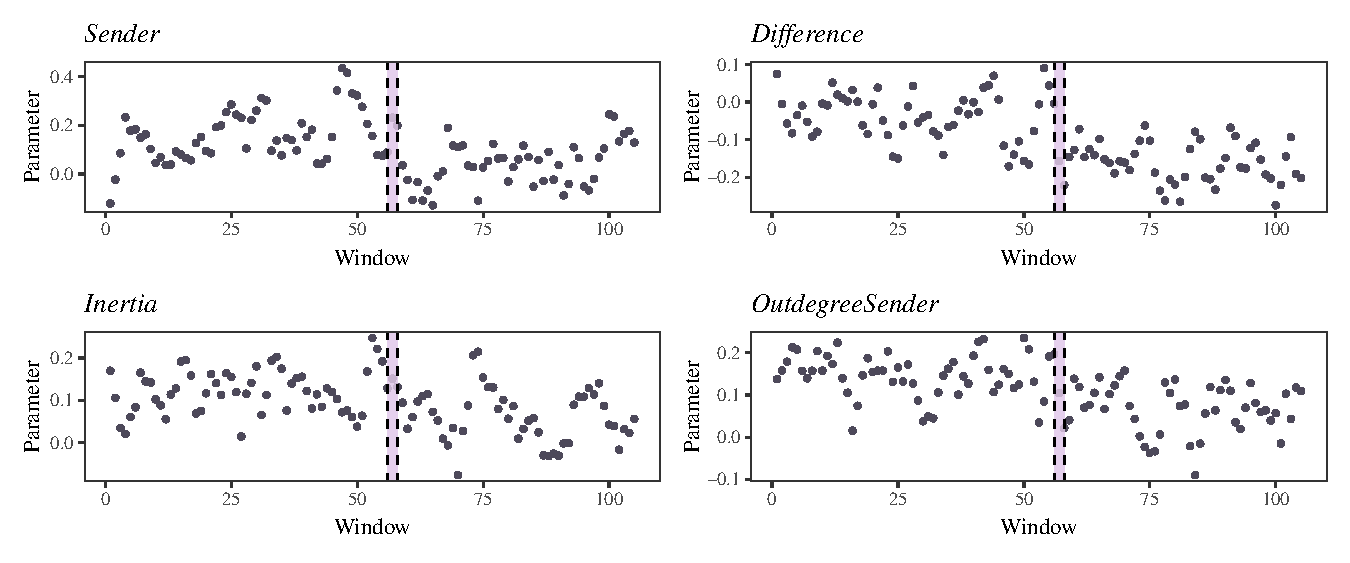
\includegraphics[width=\textwidth,height=\textheight,keepaspectratio]{parameter_wave_ex}
    	\caption{\fontsize{8}{10}\selectfont An example of a synthetic dataset after fitting the MW-REM with a window length of 2000 seconds and $\frac{2}{3}$ overlap, and extracting the effects parameters from windows. The purple block represents the interval of true changepoint windows. The y-axes indicate the effect parameter values, the x-axes represent the order of the windows along the event history. This example is based on the first synthetic dataset in the ``All of the effects have 1 changepoint'' setting.}
    	\label{parameter_wave_example}
    \end{figure}

    \subsubsection{Real-life REH data} \label{sec:Apollo 13 intro}
    
    \hspace{0.2cm} To validate the effectiveness of the three changepoint detection algorithms in practical use with MW-REM and verify their properties derived from synthetic data, we applied all three algorithms to real-life data. Specifically, we analyzed the publicly available Apollo 13 voice loop data, which recorded the communication between the astronauts and Mission Control during the failed Apollo 13 mission. The mission was intended to land on the Moon, but an agitation of one of the oxygen tanks caused an explosion that damaged the wire insulation inside, leading to the discharge of both oxygen tanks. This left the astronauts without systems to generate electricity and oxygen, forcing them to contact Mission Control for assistance and ultimately leading to the mission's cancellation. For our analysis, we selected a subset of the voice loop data covering the period from one hour before the emergency until Apollo 13 was safely back on a trajectory towards Earth. Our focus was on the relevant communication data from the mission timeline between 54:46:28 and 62:06:53 (hh:mm:ss). \\
    
    In the Apollo 13 voice loop data, a pivotal moment occurred when an astronaut stated, ``I believe we've had a problem here,'' at 55:55:21. This moment marks the start of the emergency, and we have selected it as the potential location of the changepoint in our study. We hypothesize that the old interaction patterns were disrupted after this point, making it an ideal location to test the effectiveness of the three changepoint detection algorithms on a real social network. \\
    
    For fitting the MW-REM and conducting the changepoint detection work (see the steps in Algorithm \autoref{Algorithm1}), we selected seven effects that shape the network. The first four effects are the "Inertia effect," which refers to the tendency of actors to repeatedly interact with each other, the "Outdegree of the sender effect," which refers to the tendency of actors to send events if they have sent more past events, the "Indegree of the receiver effect," which refers to the tendency of actors to receive events if they have received more past events, and the "Total degree of the sender effect," which refers to the tendency of actors to send events if they have sent and received more past events. We selected these four effects as they provide a view that captures longer-term social interactions between actors rather than immediate feedback. For this reason, we also selected three other effects that capture the patterns of immediate feedback of interactions between actors: the "AB-BA pshift," which refers to the tendency for immediate reciprocation where the next sender is the current receiver and the next receiver is the current sender, the "AB-XA pshift," which refers to the tendency for turn usurping where the next sender is not in the current event and the next receiver is the current sender, and the "AB-BY pshift," which refers to the tendency for turn receiving where the next sender is the current receiver and the next receiver is not in the current event. \\
    
    Considering the findings of Meijerink-Bosman's 2022 research \cite{meijerink-bosmanDynamicRelationalEvent2022}, we decide to fit the MW-REM with a 1000-second window length and $\frac{2}{3}$ overlap, as it provided a good insight into the dynamic of the social network. We then apply this window setting to the Apollo 13 voice loop data, extract the parameters of each effect along the windows, and feed them to the three changepoint detection algorithms employed in our study.

	\subsection{Evaluation strategies} \label{sec:evaluation method}
	
	\hspace{0.28cm} In this section, we describe how we evaluated and compared the performance of three changepoint detection algorithms applied to the extracted parameters from windows of the synthetic datasets, utilizing three metrics: (1) the confusion matrix, (2) mean squared error (MSE), and (3) mean signed difference (MSD). Our analysis focuses on evaluating the algorithms' performance across different conditions of changepoint numbers, which include no changepoint, one changepoint, and two changepoints. The classification of the synthetic data is shown in section \ref{data cate}.
	
	\subsubsection{Confusion matrix} \label{sec:confusion matrix}
	
	\hspace{0.28cm} After feeding the changepoint detection algorithms with the effects' parameters, we used the confusion matrix to evaluate the performance of each algorithm for each effect. A true positive indicates that the algorithm correctly detected a window containing the changepoint of the effect. Notably, due to the overlapping property of the windows, a changepoint can be contained in three consecutive windows simultaneously. These windows are referred to as ``changepoint windows". Therefore, if an algorithm detects the changepoint in any of these windows, it is considered a true positive. However, since the synthetic datasets are produced based on selecting the $(s,r)$ pair with the highest rate probability in the risk set $R$ for every event, the locations of the changepoints may differ slightly from our assignment. As a result, if a changepoint detection algorithm detects a changepoint within the range of three windows of the windows containing the true changepoint, we consider it a true positive. \\
	
	A false positive indicates that the algorithm falsely detected a window as a changepoint window (i.e., a window containing a changepoint), while a false negative indicates that the algorithm failed to detect a window containing the changepoint of the effect. Since our synthetic datasets are highly imbalanced, with many windows but few containing changepoints, we did not consider true negatives. \autoref{Table 3} presents the confusion matrix for changepoint detection, showing the actual and detected changepoints and non-changepoints.
	
	\begin{table}[H]
	\captionsetup{justification=raggedright, singlelinecheck=true, labelfont={bf}, labelsep=space, font={footnotesize}, width=0.85\linewidth}
	\centering
	\renewcommand{\arraystretch}{1.5} % increase cell height by 50%
	\small
	\caption{Confusion Matrix for changepoint detection}
	\begin{tabular}{l|c|c}
		\hline
		& \textit{Actual Changepoint} & \textit{Actual Non-changepoint}                   \\ \hline
		\textit{Detected Changepoint} & True Positive              & False Positive                               \\ \hline
		\textit{Detected Non-changepoint} & False Negative             & \multicolumn{1}{l}{\cellcolor[HTML]{C0C0C0}} \\ \hline
	\end{tabular}
	\label{Table 3}
    \end{table}
	
	Given the information from the confusion matrix, we employ three indicators to assess the effectiveness and performance of the three changepoint detection algorithms in detecting changepoints in REH. The first indicator is the number of false positive cases. We separately sum the number of false positives of the effects in no changepoint, one changepoint, and two changepoints conditions for each changepoint detection algorithm. For instance, for the setting of the REH with no changepoint for all effects, the number of false positives of each effect in this setting by a changepoint detection algorithm is summed in the no changepoint condition. This is done to determine which of the three changepoint algorithms has the highest likelihood of falsely detecting a changepoint when there is none, considering the no changepoint, one changepoint, and two changepoints situations in the REH. \\
	
	The second indicator is the recall. Similar to the false positives indicator, we determine the performance of the changepoint detection algorithms based on the changepoint conditions. However, since there are no true positives for the effects with no changepoint, we only consider the conditions with one and two changepoints for each changepoint detection algorithm. The recall is calculated as
	
	\begin{equation} \label{7}
		Recall_g = \frac{TP_g}{TP_g + FN_g},
	\end{equation}
    where $TP$ indicates the number of true positive cases, $FN$ indicates the number of false negative cases, and $g$ indicates the changepoint condition. Through the recall, we obtain information about the probability that each changepoint detection algorithm correctly detects the true positive for the effects with one or two changepoints, respectively, among all positive observations. \\

    The third indicator is the precision. Similar to recall, we assess the performance of the changepoint detection algorithms on precision in the one changepoint and two changepoint conditions. The precision is calculated as
 
    \begin{equation} \label{8}
    	Precision_g = \frac{TP_g}{TP_g + FP_g},
    \end{equation}
	where $TP$ represents the number of true positive cases, $FP$ represents the number of false positive cases, and $g$ represents the changepoint condition. The precision indicates the probability that a detected changepoint is indeed a changepoint, providing insight into the accuracy of the changepoint detection algorithms.
	
	\subsubsection{Mean Squared Error (MSE) \& Mean Signed Difference (MSD)} \label{sec:MSE MSD}
	
	\hspace{0.28cm} We use mean squared error (MSE) and mean signed difference (MSD) as measures to examine the accuracy of the detected changepoint window and the tendency of the algorithm to detect changepoints early or late. \\
	
	The MSE measures the average squared distance between the detected and actual changepoint windows for each changepoint detection algorithm. We compute the MSE only for true positive cases from the confusion matrix of each effect. Specifically, we calculate the MSE as \cite{aminikhanghahiSurveyMethodsTime2017}
	
	\begin{equation} \label{9}
		MSE = \frac{\sum_{i = 1}^{\#CP} (Detected(CP) - Actual(CP))^2}{\#CP},
	\end{equation}
	where $CP$ denotes the changepoint window, and $\#CP$ represents the number of changepoints in the REH. A lower MSE indicates that the algorithm's detected changepoint window is closer to the true one in general. For the MSE evaluation, we assess the performance of the changepoint detection algorithms in the one-changepoint and two-changepoint conditions. We report the average MSE of each condition for each algorithm using the formula
	
	\begin{equation} \label{10}
		Avg.MSE_g = \frac{\sum_{i=1}^{N_g} MSE_i}{N_g},
	\end{equation}
	where $Avg.MSE_g$ represents the average MSE for changepoint condition $g$, $MSE_i$ is the MSE value for the $i$th effect in changepoint condition $g$, and $N_g$ is the number of effects in changepoint condition $g$. \\
	
	The MSD, on the other hand, is used to examine the tendency of the changepoint detection algorithm to detect changepoint windows early or late. We compute the MSD only for true positive cases from the confusion matrix of each effect. Specifically, we calculate the MSD as
	
	\begin{equation} \label{11}
		MSD = \frac{\sum_{i = 1}^{\#CP} (Detected(CP) - Actual(CP))}{\#CP},
	\end{equation}
	here, a negative MSD indicates that the changepoint detection algorithm tends to detect the changepoint window earlier than the true changepoint window, while a positive MSD indicates that the algorithm tends to detect the changepoint window later than the true changepoint window. To calculate the MSD of each changepoint detection algorithm on different changepoint conditions, we compute the average MSD, which is given by
	
	\begin{equation} \label{12}
		Avg.MSD_g = \frac{\sum_{i=1}^{N_g} MSD_i}{N_g},
	\end{equation}
	where $Avg.MSD_g$ represents the average MSD for changepoint condition $g$, $MSD_i$ is the MSD value for the $i$th effect in changepoint condition $g$, and $N_g$ is the number of effects in changepoint condition $g$. This allows us to assess each changepoint detection algorithm's tendency to detect changepoint windows early or late in both univariate and multivariate changepoints scenarios of effects.
	
	\section{\fontsize{14}{15}\selectfont Results \& Discussion} \label{sec:results}
	
	\subsection{Synthetic REH data} \label{res:simulation}
	
	\hspace{0.28cm} In this section, we present the results of the changepoint detection analysis conducted on the synthetic REH data. We summarize the performance of three changepoint detection algorithms under zero, one, and two changepoint conditions based on the following metrics: (1) the number of false positives, (2) recall, (3) precision, (4) average MSE, and (5) average MSD.
	
	\begin{figure}[H]
		\captionsetup{justification=raggedright}
		\captionsetup{labelfont={bf}, labelsep=space, font={footnotesize}}
		\renewcommand{\figurename}{Figure}
		\centering
		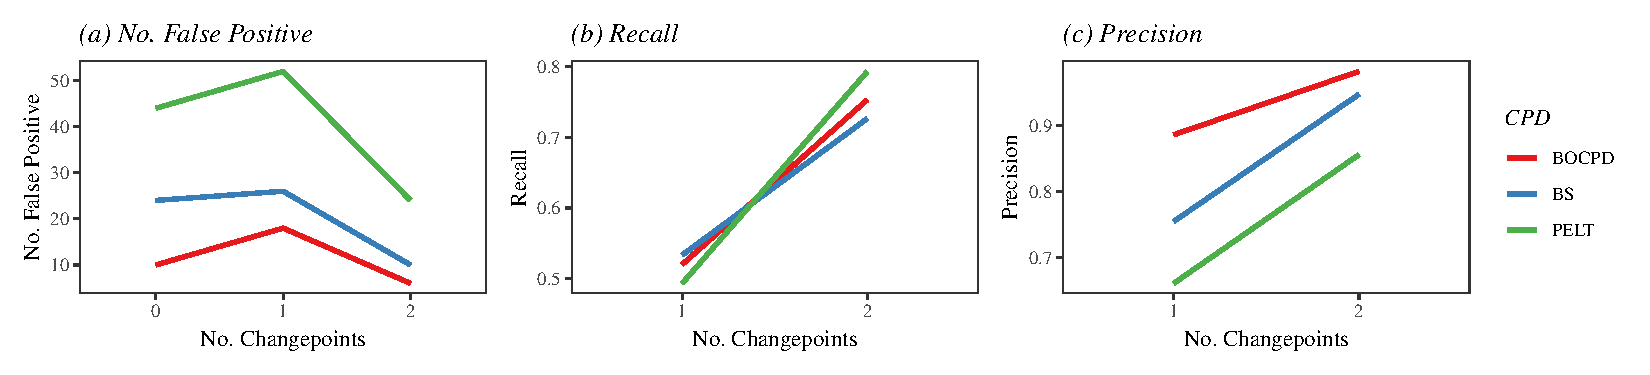
\includegraphics[width=\textwidth,height=\textheight,keepaspectratio]{FPTPRPPV}
		\caption{\fontsize{8}{10}\selectfont The plot displays the (a) number of false positives, (b) recall, and (c) precision of the three changepoint detection algorithms under no changepoint, one changepoint, and two changepoints conditions. The y-axes indicate the values of interest, the x-axes indicate the different changepoint conditions. The red line represents BOCPD, the blue line represents BS, and the green line represents PELT.}
		\label{Figure 3}
	\end{figure}
	
	The results of the simulation studies demonstrate the effectiveness of all three changepoint detection algorithms (BS, PELT, and BOCPD). In \autoref{Figure 3} (a), we observe the overall performance of the algorithms in terms of false positives. The BOCPD algorithm outperforms the other algorithms in all scenarios. This suggests that the BOCPD algorithm has a better ability to correctly identify windows that are not changepoint windows in any situation. Conversely, the PELT algorithm is the most prone to incorrectly identify non-changepoint windows as changepoint windows. \\
	
	Regarding the recall in \autoref{Figure 3} (b), all three changepoint detection algorithms have similar recall values in the univariate changepoint condition, which are around 0.5. This indicates that if an effect has only one changepoint throughout the entire REH, the probability of detecting the window within a range of three windows from the true one is around 50\%, using any of the three algorithms. In the case of the multivariate changepoint condition, all three algorithms show significant improvement, especially PELT, which almost reaches 80\%. \\
	
	In \autoref{Figure 3} (c), we present the precision performance of the three algorithms. As with recall, all three algorithms show improved precision in the multivariate changepoint condition, with each achieving a precision of over 0.85. BOCPD consistently performs at a high level, regardless of the changepoint condition. This suggests that the changepoint windows it identified are highly likely to be the windows within three windows' range of the true changepoint window. The low precision and high recall of PELT, however, are a trade-off with its high false positives. PELT detects more changepoint windows, which increases the likelihood of covering more true positives in its detections, but at the same time, the high false positives result in the lowest precision among the three algorithms. Details of the performance of each algorithm in terms of the three metrics are shown in \autoref{FN_TPR_PPV}.
	
	\begin{table}[H]
		\captionsetup{justification=raggedright, singlelinecheck=true, labelfont={bf}, labelsep=space, font={footnotesize}, width=0.65\linewidth}
		\captionsetup{labelfont={bf}, labelsep=space, font={footnotesize}}
		\centering
		\renewcommand{\arraystretch}{1.2} % increase cell height by 50%
		\small
		\caption{False negatives, recall, and precision for each changepoint detection algorithm in various changepoint conditions.}
		\begin{tabular}{lccc}
			\hline
			& \textit{BS} & \textit{PELT} & \textit{BOCPD} \\ \hline
			\textbf{Number of false negatives} &             &               &                \\
			\textit{No changepoint condition}   & 24          & 44            & 10             \\
			\textit{One changepoints condition} & 26          & 52            & 18             \\
			\textit{Two changepoints condition} & 10          & 24            & 6              \\
			\textbf{Recall}                    &             &               &                \\
			\textit{One changepoints condition} & 0.53        & 0.49          & 0.52           \\
			\textit{Two changepoints condition} & 0.73        & 0.79          & 0.75           \\
			\textbf{Precision}                 &             &               &                \\
			\textit{One changepoints condition} & 0.75        & 0.66          & 0.89           \\
			\textit{Two changepoints condition} & 0.95        & 0.86          & 0.98           \\ \hline
		\end{tabular}
	\label{FN_TPR_PPV}
	\end{table}

    \begin{figure}[H]
    	\captionsetup{justification=raggedright}
    	\captionsetup{labelfont={bf}, labelsep=space, font={footnotesize}}
    	\renewcommand{\figurename}{Figure}
    	\centering
    	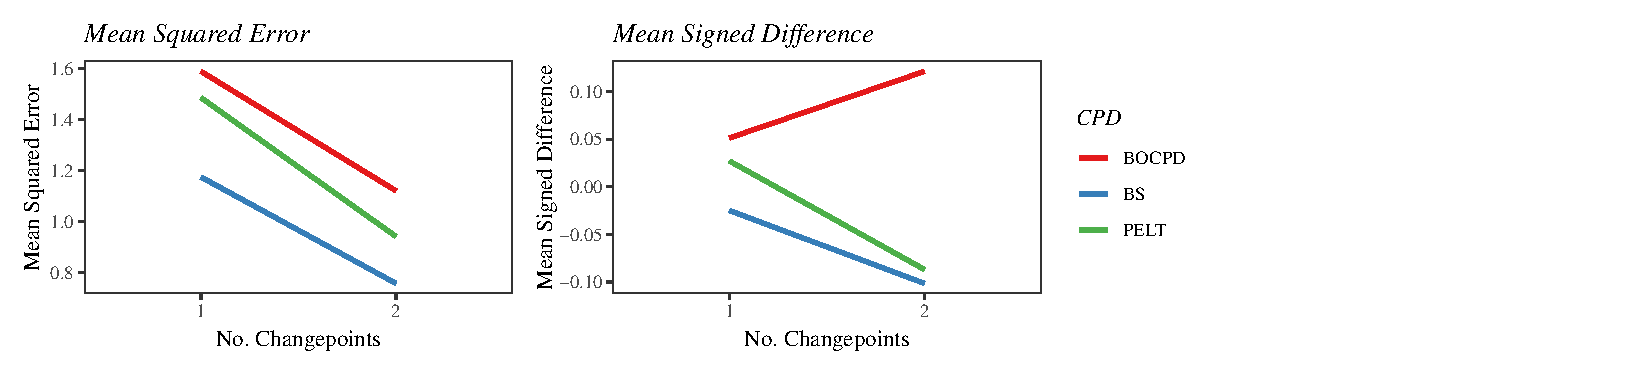
\includegraphics[width=10cm]{MSEMSD}
    	\caption{\fontsize{8}{10}\selectfont The plot shows the (a) average mean squared error, and (b) average mean signed difference under no changepoint, one changepoint, and two changepoints conditions. The y-axes indicate the values of interest, the x-axes indicate the different changepoint conditions. The red line represents BOCPD, the blue line represents BS, and the green line represents PELT.}
    	\label{Figure 4}
    \end{figure}

    Regarding the quality of the true positive windows for each algorithm, we used average MSE as a criterion. In \autoref{Figure 4} (a), we present the average MSE performance of the three algorithms. The average MSE measures the average squared distance between the detected and actual changepoint windows for different changepoint situations. A lower MSE value indicates that the detected true positive changepoint windows are closer to the true changepoint windows. Among the three algorithms, BS performs the best in both univariate and multivariate changepoint situations, with the lowest average differences between its detected and actual changepoint windows. However, the differences between the three algorithms are small overall. \\
    
    \autoref{Figure 4} (b) reveals the average MSD of each algorithm. The average MSD provides information about the average relative location of the detected changepoint window with the true changepoint window in different changepoint situations for each algorithm. The BOCPD tends to detect the changepoint window after the true changepoint, whether in the univariate or multivariate changepoint context. In contrast, the BS tends to detect the window before the true changepoint, and PELT has mixed performance. The reason why BS and PELT tend to detect the changepoint window before the true changepoint is that they merge small intervals based on a cost function balancing data likelihood and model complexity \cite{killickOptimalDetectionChangepoints2012}. This approach favors fewer, larger changepoints and may lead to detecting changepoints slightly before the true location \citealp{fearnheadChangepointDetectionPresence2019}. Additionally, it is possible that the true changepoint window is located in a region of the time series where the effect parameters are already changing but have not yet fully transitioned to the new regime. Details of the performance of each algorithm in terms of the average MSE and average MSD metrics are shown in \autoref{Avg_MSEMSD}.

    \begin{table}[H]
    	\captionsetup{justification=raggedright, singlelinecheck=false, labelfont={bf}, labelsep=space, font={footnotesize}, width=0.63\linewidth}
    	\captionsetup{labelfont={bf}, labelsep=space, font={footnotesize}}
    	\centering
    	\renewcommand{\arraystretch}{1.2} % increase cell height by 50%
    	\small
    	\caption{Average MSE and average MSD for each changepoint detection algorithm in various changepoint conditions.}
    	\begin{tabular}{lccc}
    		\hline
    		& \textit{BS} & \textit{PELT} & \textit{BOCPD} \\ \hline
    		\textbf{Average MSE}               &             &               &                \\
    		\textit{One changepoints condition} & 1.18        & 1.49          & 1.59           \\
    		\textit{Two changepoints condition} & 0.76        & 0.94          & 1.12           \\
    		\textbf{Average MSD}               &             &               &                \\
    		\textit{One changepoints condition} & -0.03       & 0.03          & 0.05           \\
    		\textit{Two changepoints condition} & -0.1        & -0.09          & 0.12          \\ \hline
    	\end{tabular}
    	\label{Avg_MSEMSD}
    \end{table}

    Overall, the BOCPD performs well in terms of precision; the changepoint windows identified by the BOCPD are highly likely to contain the true changepoints or within a three-window range of the true changepoint windows. However, in general, it cannot detect as many true changepoint windows as PELT. PELT has good performance on recall; the true changepoint windows are likely to be covered by all the detected changepoint windows from PELT. However, this comes at the cost of high false positives and low precision. The BS performs well in terms of average MSE; the location of its detected changepoint windows is usually close to the true changepoint window if the detected changepoint windows are true positive cases (i.e., within the three-window range of the true changepoint windows). However, the weakness of the BS is that it has the lowest recall among the three algorithms, which can cause it to miss detecting certain changepoint windows. Moreover, in practice, it is challenging to determine whether a detected changepoint window is a true positive or not. Therefore, instead of relying solely on the BS, we suggest using it in conjunction with other algorithms. By comparing the nearby detected changepoint windows between the BS and other algorithms, we can identify the true positive changepoint windows and choose the window detected by the BS as it has good performance in terms of average MSE. Below shows the suitable application scenarios of each algorithm:
    
    \begin{itemize}
    	\item BS: suitable when accurately identifying the location of the changepoint window is essential. Note that this algorithm needs to be used in conjunction with other algorithms as an auxiliary tool. \\
    	
    	\item PELT: appropriate when it is critical to identify all potential changepoint windows, even if it means a higher likelihood of false positives. \\
    	
    	\item BOCPD: recommended when proper identification of changepoint windows is crucial and minimizing the number of incorrect detections is a priority, even if it means potentially missing some true changepoint windows.
    \end{itemize}
    
    On the other hand, it is worth noting that all three algorithms perform better on multivariate changepoint conditions (i.e., scenarios with more than one changepoint) in all the metrics we employed. This is because detecting multiple changepoints can provide more information about the underlying structure of the data. Conversely, detecting one or fewer changepoints may not provide enough information to distinguish between random fluctuations and actual changes \cite{liReviewChangepointDetection2019}.
    
	\subsection{Real-life REH data} \label{res:Apollo 13}
	
	\hspace{0.28cm} We validated the feasibility of integrating changepoint detection algorithms and MW-REM. Additionally, we confirmed our simulation analysis findings using real-life data from the Apollo 13 voice loop. The emergency report for Apollo 13 occurred at $t$ = 55:55:21 (hh:mm:ss). We applied the MW-REM with a window length of 1000 seconds and $\frac{2}{3}$ overlap, resulting in a total of 76 windows. The potential changepoint window for our study corresponds to the window from 9 to 11, covering the time slot from 55:38:53 to 56:06:40. \\
	
	\begin{figure}[H]
		\captionsetup{justification=raggedright}
		\captionsetup{labelfont={bf}, labelsep=space, font={footnotesize}}
		\renewcommand{\figurename}{Figure}
		\centering
		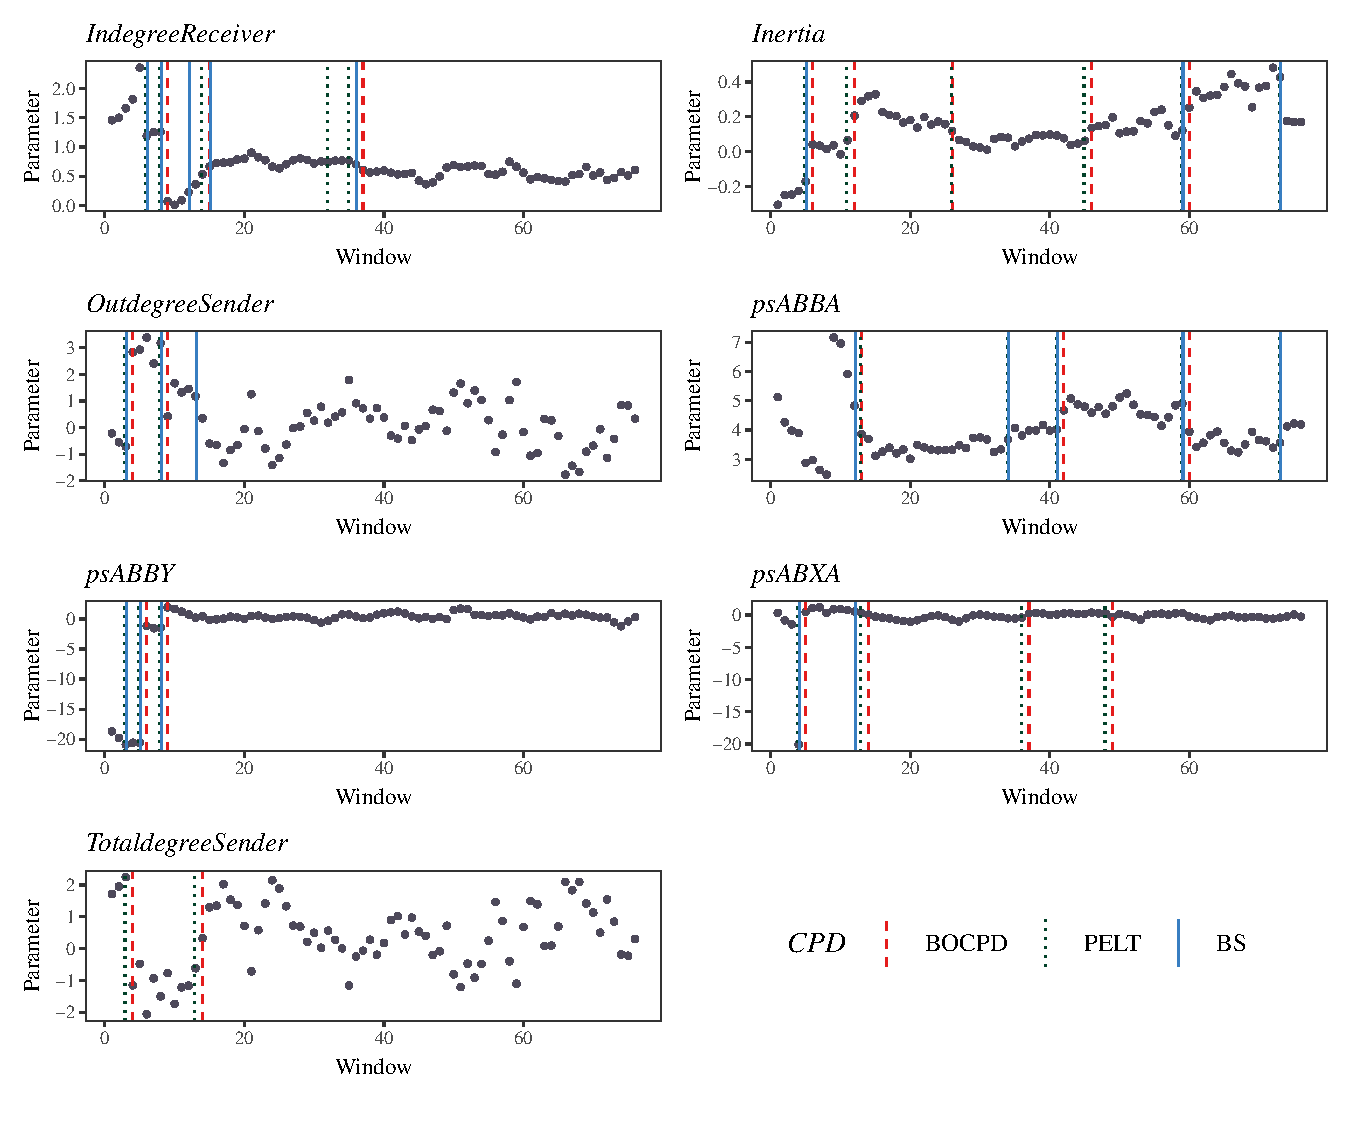
\includegraphics[width=\textwidth,height=\textheight,keepaspectratio]{Apollo_CPD_bw}
		\caption{\fontsize{8}{10}\selectfont The changepoint detection results of the three algorithms. The red dashed line represents BOCPD, the green dotted line represents PELT, the blue solid line represents BS. The y-axes indicate the effect parameter values, the x-axes represent the order of the windows along the event history.}
		\label{Apollo_effects_cp_plot}
	\end{figure}

    \begin{table}[H]
    	\captionsetup{justification=raggedright, singlelinecheck=true, labelfont={bf}, labelsep=space, font={footnotesize}, width=0.95\linewidth}
    	\captionsetup{labelfont={bf}, labelsep=space, font={footnotesize}}
    	\centering
    	\renewcommand{\arraystretch}{1.2} % increase cell height by 50%
    	\small
    	\caption{The changepoint detection results of the three algorithms.}
    	\begin{tabular}{lccc}
    		\hline
    		& \textit{BS}        & \textit{PELT}         & \textit{BOCPD}                   \\ \hline
    		\textit{IndegreeReceiver}  & 6, 8, 12, 15, 36   & 6, 8, 14, 32, 35      & {\color[HTML]{000000} 9, 15, 37} \\
    		\textit{Inertia}           & 5, 59, 73          & 5, 11, 26, 45, 59, 73 & 6, 12, 26, 46, 60                \\
    		\textit{OutdegreeSender}   & 3, 8, 13           & 3, 8                  & 4, 9                             \\
    		\textit{psABBA}            & 12, 34, 41, 59, 73 & 13, 34, 41, 59, 73    & 13, 42, 60                       \\
    		\textit{psABBY}            & 3, 5, 8            & 3, 5, 8               & 6, 9                             \\
    		\textit{psABXA}            & 4, 12              & 4, 13, 36, 48         & 5, 14, 37, 49                    \\
    		\textit{TotaldegreeSender} & None               & 3, 13                 & 4, 14                            \\ \hline
    	\end{tabular}
    	\label{Apollo_effects_cp}
    \end{table}
	
	We inputted the effect parameters obtained from the MW-REM windows into three different changepoint detection algorithms: BOCPD, BS, and PELT. The resulting changepoint detections are displayed in \autoref{Apollo_effects_cp_plot} and \autoref{Apollo_effects_cp}. As the emergency occurred between windows 9 and 11, we anticipated that the algorithms would detect the emergency during or around that time frame. \\
	
	Among the three changepoint detection algorithms, BOCPD detected the window containing the emergency report most accurately, pinpointing the exact window of the emergency at the indegree of the receiver effect, outdegree of the sender effect, and the AB-BA pshift effect. PELT identified the window involving the emergency report once at the inertia effect. However, none of the detections from BS correctly identified the window including the emergency report. Nonetheless, detecting the changepoint window slightly after the window that contained the emergency can also be justified. The MW-REM focuses on the communication dynamics between actors, in this case, the astronauts and Mission Control. It is plausible that their communication patterns did not immediately change after the emergency occurred but rather shifted after some time had passed. In this study, BS was able to capture the windows within two windows after the emergency window in four effects, while PELT and BOCPD both detected the windows within three windows after the emergency window in four effects. \\
	
	On the other hand, BS and PELT algorithms sometimes tend to detect the changepoint window slightly before the actual changepoint window due to their interval merging property. Furthermore, our study is a retrieval study that analyzed the complete data rather than updated data over time, which could have led the algorithms to detect the changepoint window slightly earlier. Thus, in our study, we observed that both BS and PELT identified one window before the emergency window as a changepoint window in three effects: the indegree of the receiver effect, outdegree of the sender effect, and AB-BY pshift effect. \\
	
	It is also worth noting that the algorithms identified changepoint windows at around windows 35 and 40 in multiple effects, such as the indegree of the receiver effect, the AB-BA pshift effect, and the AB-XA pshift effect. We found that this was because the oxygen level in the tanks was insufficient to support the operation of the command and service module between the time frames of 58:03:20 and 58:20:00 (i.e., window 35). To address this issue, the astronauts and Mission Control decided to turn off the command and service module and use the lunar module instead, with these actions taking place between the time frames of 58:31:06 and 59:04:26 (i.e., windows 40 to 42). In addition, the algorithms commonly identified windows around 60 and 73 as changepoint windows in the inertia effect and AB-BA pshift effect. It was found that they encountered a water shortage crisis between 60:16:40 and 60:44:26 (i.e., window 59 to 61), and to save water usage, Mission Control suggested turning off the Apollo’s primary guidance, navigation, and control system, which was done around 61:34:26 to 61:51:06 (i.e., window 73). \\
	
	Overall, the Apollo 13 data provided further confirmation of the effectiveness of the three algorithms when applied to MW-REM, as well as the findings of our simulation study regarding changepoint detection. All three algorithms we used performed well, identifying the changepoints either at or near the window that contained the emergency report for almost all effects. BOCPD had high precision and detected only a small number of changepoint windows, mostly the emergency report windows. PELT had the best recall performance among the three algorithms but detected a larger number of changepoint windows, including those around or at the emergency report windows for all effects. BS had the worst recall performance and did not detect any changepoint windows around the emergency for the inertia effect and total degree of the sender effect, while BOCPD and PELT did. However, the windows it detected near the emergency window were mostly within a very short distance from the emergency window (i.e., at most two windows distances). Furthermore, our study found that not only the hypothesized changepoint windows, but also the other detected changepoint windows were similar to the changepoints detected by Shafiee Kamalabad et al.'s study in 2023, which also utilized the Apollo 13 data for changepoint detection \cite{shafieekamalabadWhatPointChange2023}.
	
	\section{\fontsize{14}{15}\selectfont Conclusion} \label{sec:conclusion}
	
	\hspace{0.28cm} In this thesis, we investigated the effectiveness of integrating three widely used changepoint detection algorithms (BOCPD, BS, and PELT) with MW-REM, and evaluated their performance using both synthetic and real-life data from the Apollo 13 mission. Our results demonstrated that these algorithms were effective in detecting changepoints in social networks. Both the synthetic data analysis and the Apollo 13 mission analysis showed that the algorithms were able to identify most of the changepoints in the multivariate changepoint contexts of the social network. Specifically, all three algorithms had high recall in the synthetic data and were able to identify almost all the effects' windows containing or nearing the emergency report in the Apollo 13 analysis. \\
	
	BOCPD performed well in precision, tending to give fewer but mostly true changepoint windows. PELT had good recall performance but a higher number of false negative cases. BS was the least effective algorithm, it could not reveal as many true changepoint windows as PELT and also lacked the high precision of BOCPD. However, it could be a useful auxiliary tool, as it was good at identifying the location which was exact or very close to the changepoint window. It should be noted that PELT and BS sometimes detected the changepoint window slightly earlier than the actual changepoint window in the retrieval study due to their interval merging property, where they recognized a changepoint in a certain interval. \\
	
	In conclusion, our study demonstrated the effectiveness of utilizing changepoint detection algorithms within the MW-REM structure to detect changepoints in social networks. This approach has significant implications for various fields, including social science, economics, and epidemiology, as it can help identify critical changes in complex systems. While our study successfully identified the time period of changepoints, future research can build upon our work by exploring the potential of identifying the exact time point of changepoints using a combination of the changepoint detection algorithms we utilized with the Bayes factor changepoint detection method proposed by Shafiee Kamalabad et al \cite{shafieekamalabadWhatPointChange2023}. This approach has the potential to provide more precise information about when changepoints occur in the event history, which can be useful for decision-making in various applications. \\
	
	Overall, our study offered a valuable tool for identifying critical changes in social networks, and we hope that it will inspire further research in this area. By continuing to develop and refine changepoint detection methods, we can gain a deeper understanding of complex systems and make more informed decisions to improve our world. \\
	
	
	\newpage
	
	\nocite{*} % Print all the References out, not only the citing
	\bibliographystyle{abbrv}
	\bibliography{My_Library}
	
\end{document}
